\section{Review of Graph Neural Networks}

In this section, we introduce the concepts related to the graph neural network (GNN, for short) and breifly survey typical graph neural networks.
We denote a simple graph $\mathcal{G}$ as $\mathcal{G}=(\mathcal{V}, \mathcal{E})$, where $\mathcal{V}$ and $\mathcal{E}$ are the vertex set and the edge set of $\mathcal{G}$, respectively.
Let $n=|\mathcal{V}|$ and $m=|\mathcal{E}|$ as the number of vertices/edges. 
We use $v_i$ $(0 \leq i < n)$ to denote a vertex and $e_{i,j}=(v_i, v_j)$ to denote the edge pointing from $v_i$ to $v_j$.
The adjacency set of $v_i$ is $\mathcal{N}(v_i)=\{v|(v_i, v) \in \mathcal{E}\}$.
We denote a \emph{vector} with a bold lower case letter like $\boldsymbol{x}$ and a \emph{matri}x with a bold upper case letter like $\boldsymbol{X}$.

\subsection{General Structure of Graph Neural Networks}

As illustracted in \figurename~\ref{fig:general_structure_of_gnn}, a typical GNN can be decomposed into three parts: an input layer + several GNN layers + a prediction layer.

\begin{figure}
	\centering
	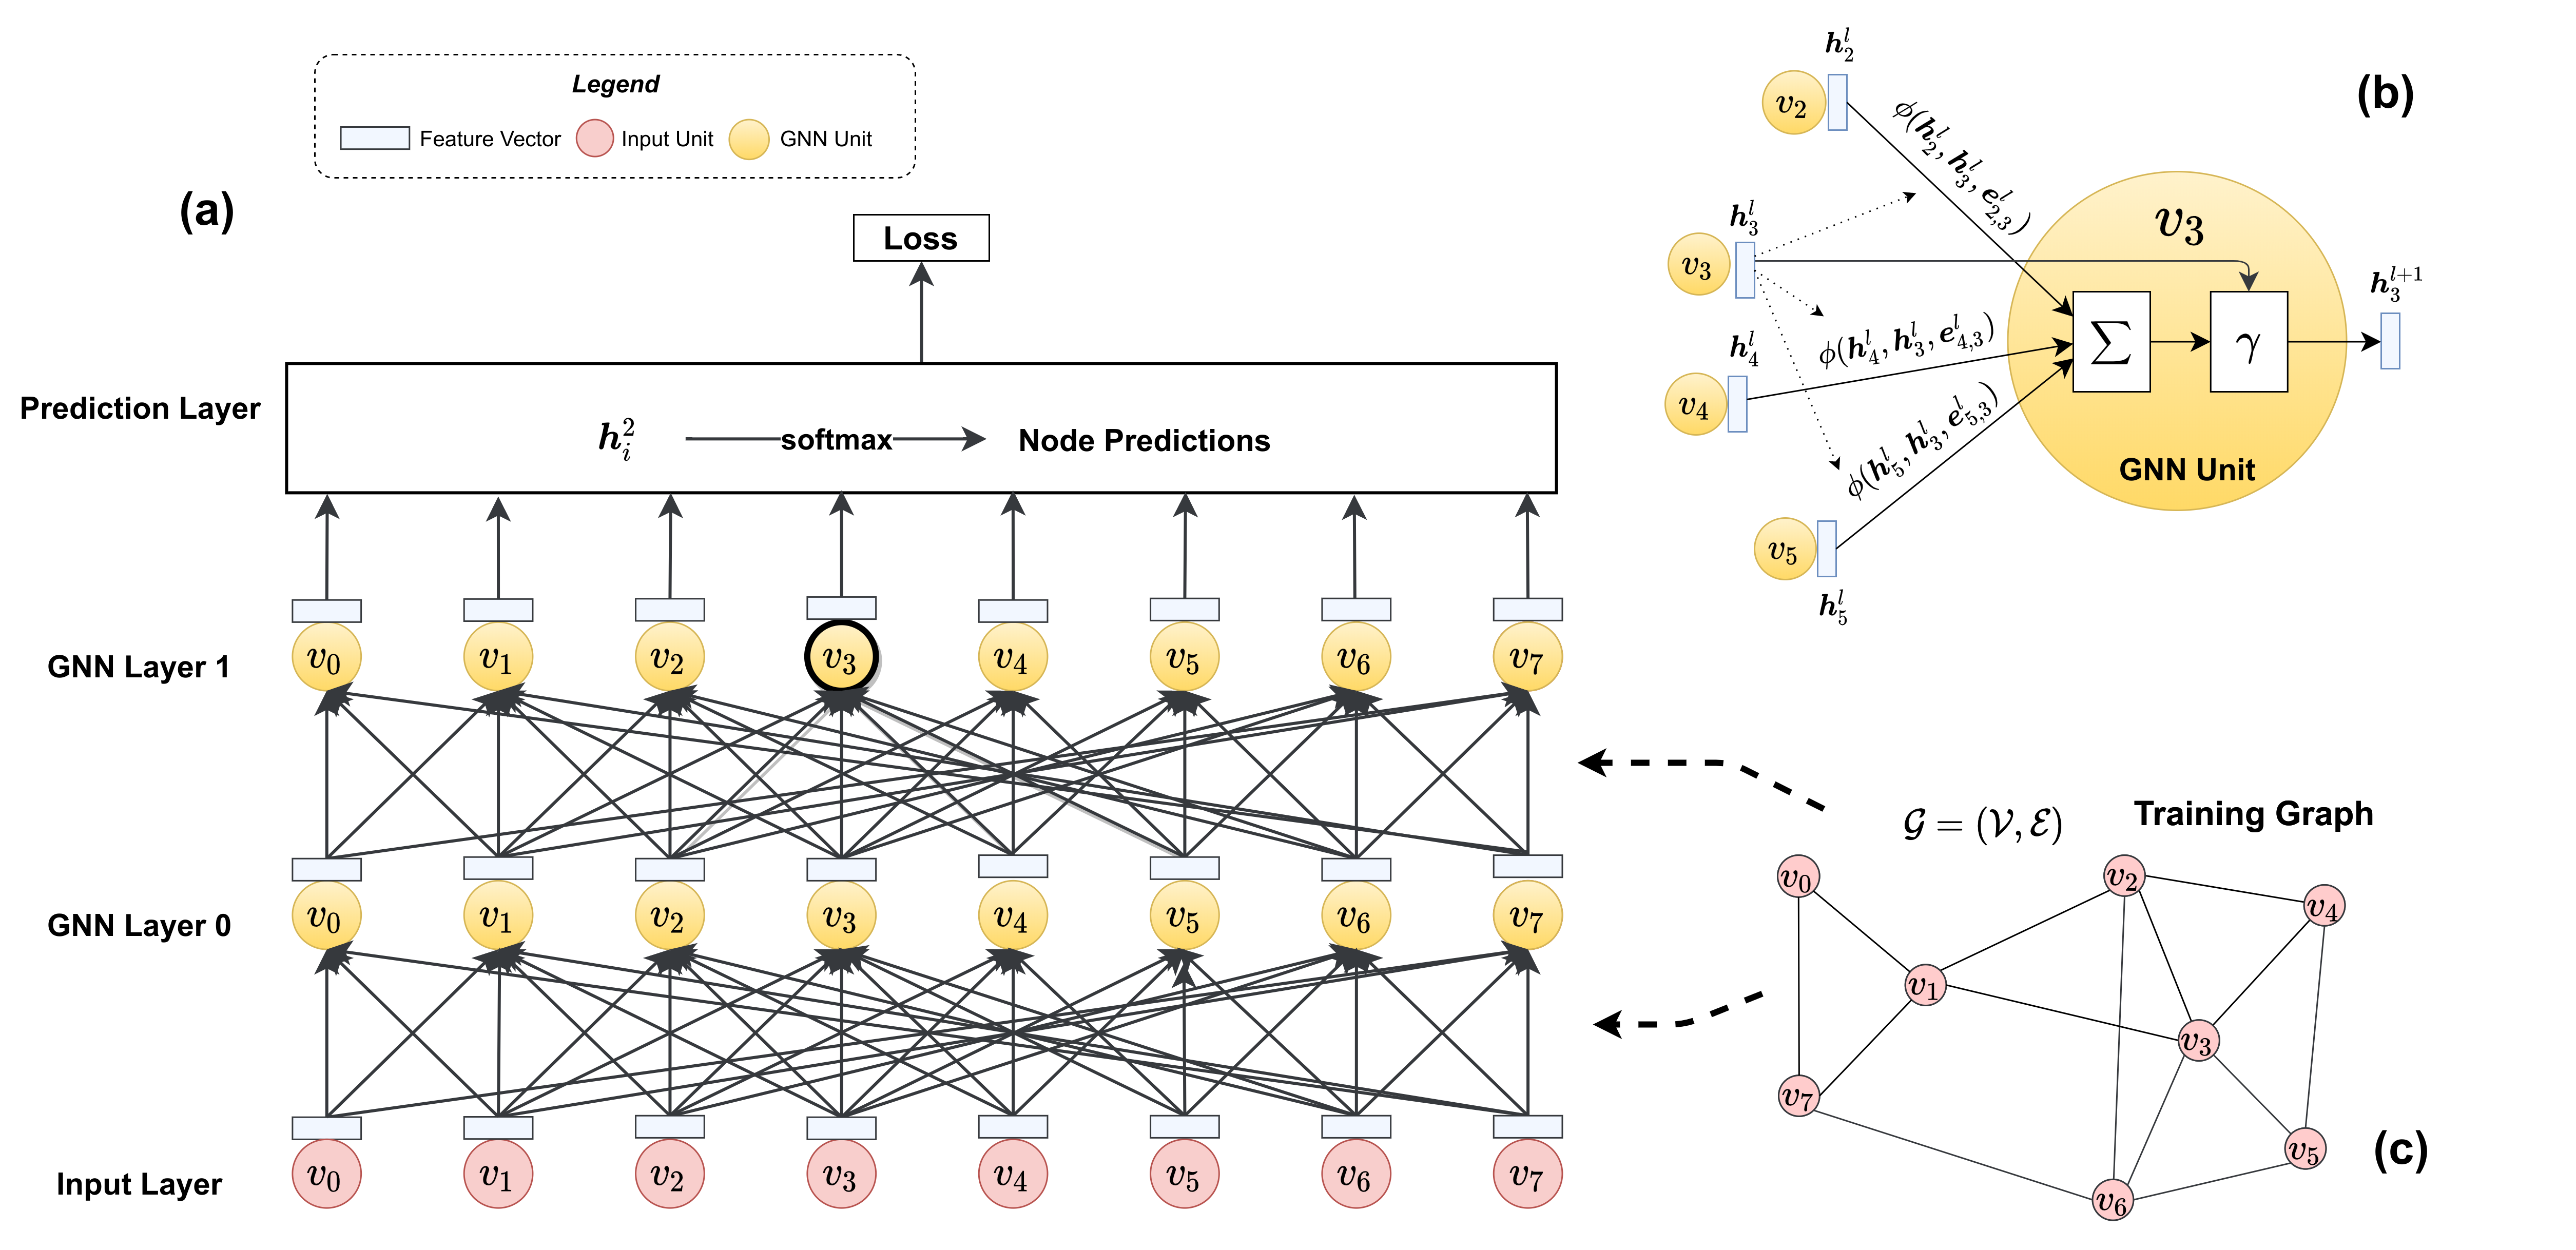
\includegraphics[width=1.1\columnwidth]{figs/illustration/GNN_common_architecture.png}
	\caption{Structure of a typical graph neural network. (a) Demo GNN, (b) Demo graph. The target application is the node classification. The demo GNN has two GNN layers.}
	\label{fig:general_structure_of_gnn}
\end{figure}

A GNN receives a graph $\mathcal{G}$ as the input.
Every vertex $v_i$ in $\mathcal{G}$ is attached with a feature vector $\boldsymbol{x}_i$ to describe the properties of the vertex.
The edges of $\mathcal{G}$ may also be attached with feature vectors $\boldsymbol{e}_{i,j}$
The input layer of a GNN receives feature vectors from all vertices and passes them to GNN layers.

A GNN layer consists of $n$ graph neurons, where $n$ is the number of vertices in $\mathcal{G}$.
Each graph neuron corresponds to a vertex in $\mathcal{G}$.
In the first GNN layer (Layer 0), the graph neuron of the vertex $v_i$ collects input feature vectors of itself and the vertices $\boldsymbol{x}_j$ that are adjacent to $v_i$ in $\mathcal{G}$ (i.e., $v_j \in \mathcal{N}(v_i)$) from the input layer.
After aggregating input feature vectors and applying non-linear transformation, the graph neuron outputs a hidden feature vector $\boldsymbol{h}^1_i$ for $v_i$.
Take the demo DNN in \figurename~\ref{fig:general_structure_of_gnn}(a) as the example.
Since $\mathcal{N}(v_3) = \{v_1, v_2, v_4, v_5, v_6\}$, the graph neuron of $v_1$ at layer 0 collects the feature vectors \{$\boldsymbol{x}_1$, $\boldsymbol{x}_2$, $\boldsymbol{x}_3$, $\boldsymbol{x}_4$, $\boldsymbol{x}_5$, $\boldsymbol{x}_6$\} from the input layer and outputs $\boldsymbol{h}^1_1$.
Different GNNs mainly differ in the graph neurons that they use.
We elaborate on their details later.

The connection between the input layer and the first GNN layer is determined by the topology of $\mathcal{G}$.
In the traditional neural networks, neurons of neighboring layers are fully connected.
In GNNs, two graph neurons are connected only if their corresponding vertices have an edge between them in $\mathcal{G}$.
Most real-world graphs are very \emph{sparse}, i.e. $|\mathcal{E}| \ll |\mathcal{V}|^2$. 


In the next GNN layer (Layer 1), the graph neuron of $v_i$ collects the hidden feature vectors of itself $\boldsymbol{h}^1_i$ and its neighbors ($\boldsymbol{h}^1_j$ with $v_j \in \mathcal{N}(v_i)$) from the \emph{previous} GNN layer.
Based on the collected hidden vectors, the graph neuron in Layer 1 outputs a new hidden feature vector $\boldsymbol{h}^2_i$ for $v_i$.
Though there are only two GNN layers in \figurename~\ref{fig:general_structure_of_gnn}, a GNN allows to stack more GNN layers to support deeper graph analysis.
%In \figurename~\ref{fig:general_structure_of_gnn}, we shows a GNN with two layers.

Assume there are $L$ GNN layers.
The last GNN layer (Layer $L-1$) outputs a hidden feature vector $\boldsymbol{h}^{L}_i$ for every vertex $v_i$.
As an embedding vector, $\boldsymbol{h}^L_i$ encodoes the knowledge learned from the input layer and all the previous GNN layers.
Since $\boldsymbol{h}^L_i$ is affected by $v_i$ and the vertices in the $L$-hop neighborhood of $v_i$, analyzing a graph with a \emph{deeper} GNN means analyzing each vertex with a \emph{wider} scope.

The hidden feature vectors $\boldsymbol{h}^L_i$ of the last GNN layer are fed to the prediction layer to generate the output of the whole GNN.
The prediction layer is a standard nerual network.
The structure of the prediction layer depends on the prediction task of the GNN.
Take the node classification task as the example, as shown in \figurename~\ref{fig:general_structure_of_gnn}.
The node classification predicts a label for every vertex in $\mathcal{G}$.
In this case, the prediction layer can be a simple softmax layer with $\boldsymbol{h}^L_i$ as the input and a vector of probabilities as the output.
If the prediction task is edge prediction, the hidden feature vectors of two vertices are concatenated and fed into a softmax layer.
If we need to predict a label for the whole graph, a pooling (max/mean/...) layer is added to generate an embedding vector for the whole graph and the embedding vector is used to produce the final prediction.

Supporting end-to-end training is a prominent advantage of GNN, compared with other graph-based machine learning methods.
We can calculate the gradients of the loss function on the model parameters from the prediction layer directly.
With the help of the back proporgation technique, the gradient is propogated from the prediction layer back to the previous GNN layers layer by layer.
The model parameters are updated with a gradient descent optimizer like Adam.
Except for the input feature vector, there is no need to conduct handworked feature extraction.
In a fully parameterized way, the GNN automatically extracts an embedding vector for each vertex from its $L$-hop neighborhood.
The parameters are tuned according to the specific prediction task, leading to high prediction accuracy.

\subsection{Graph Neuron and Message-passing Model}

Graph neurons are building blocks of a GNN.
A GNN layer consists of $|\mathcal{V}|$ graph neurons.
Each vertex corresponds to a graph neuron.
A graph neuron as shown in \figurename~\ref{fig:graph_neuron_structure} is a small neural network.
The graph neuron of $v_i$ at layer $l$ receives hidden feature vectors $\boldsymbol{h}^l_j$ from the graph neurons of $v_i$ and its neighbors ($v_j \in \{v_i\} \cup \mathcal{N}(v_i)$) at the previous GNN layer \footnote{For the GNN layer 0, graph neurons receive input feature vectors, i.e., $\boldsymbol{h}^0_i=\boldsymbol{x}_i$}.
The graph neuron aggregates the received hidden feature vectors, applies non-linear transformations, and outputs a new hidden feature vector $\boldsymbol{h}_i^{l+1}$.

\begin{figure}
	\centering
	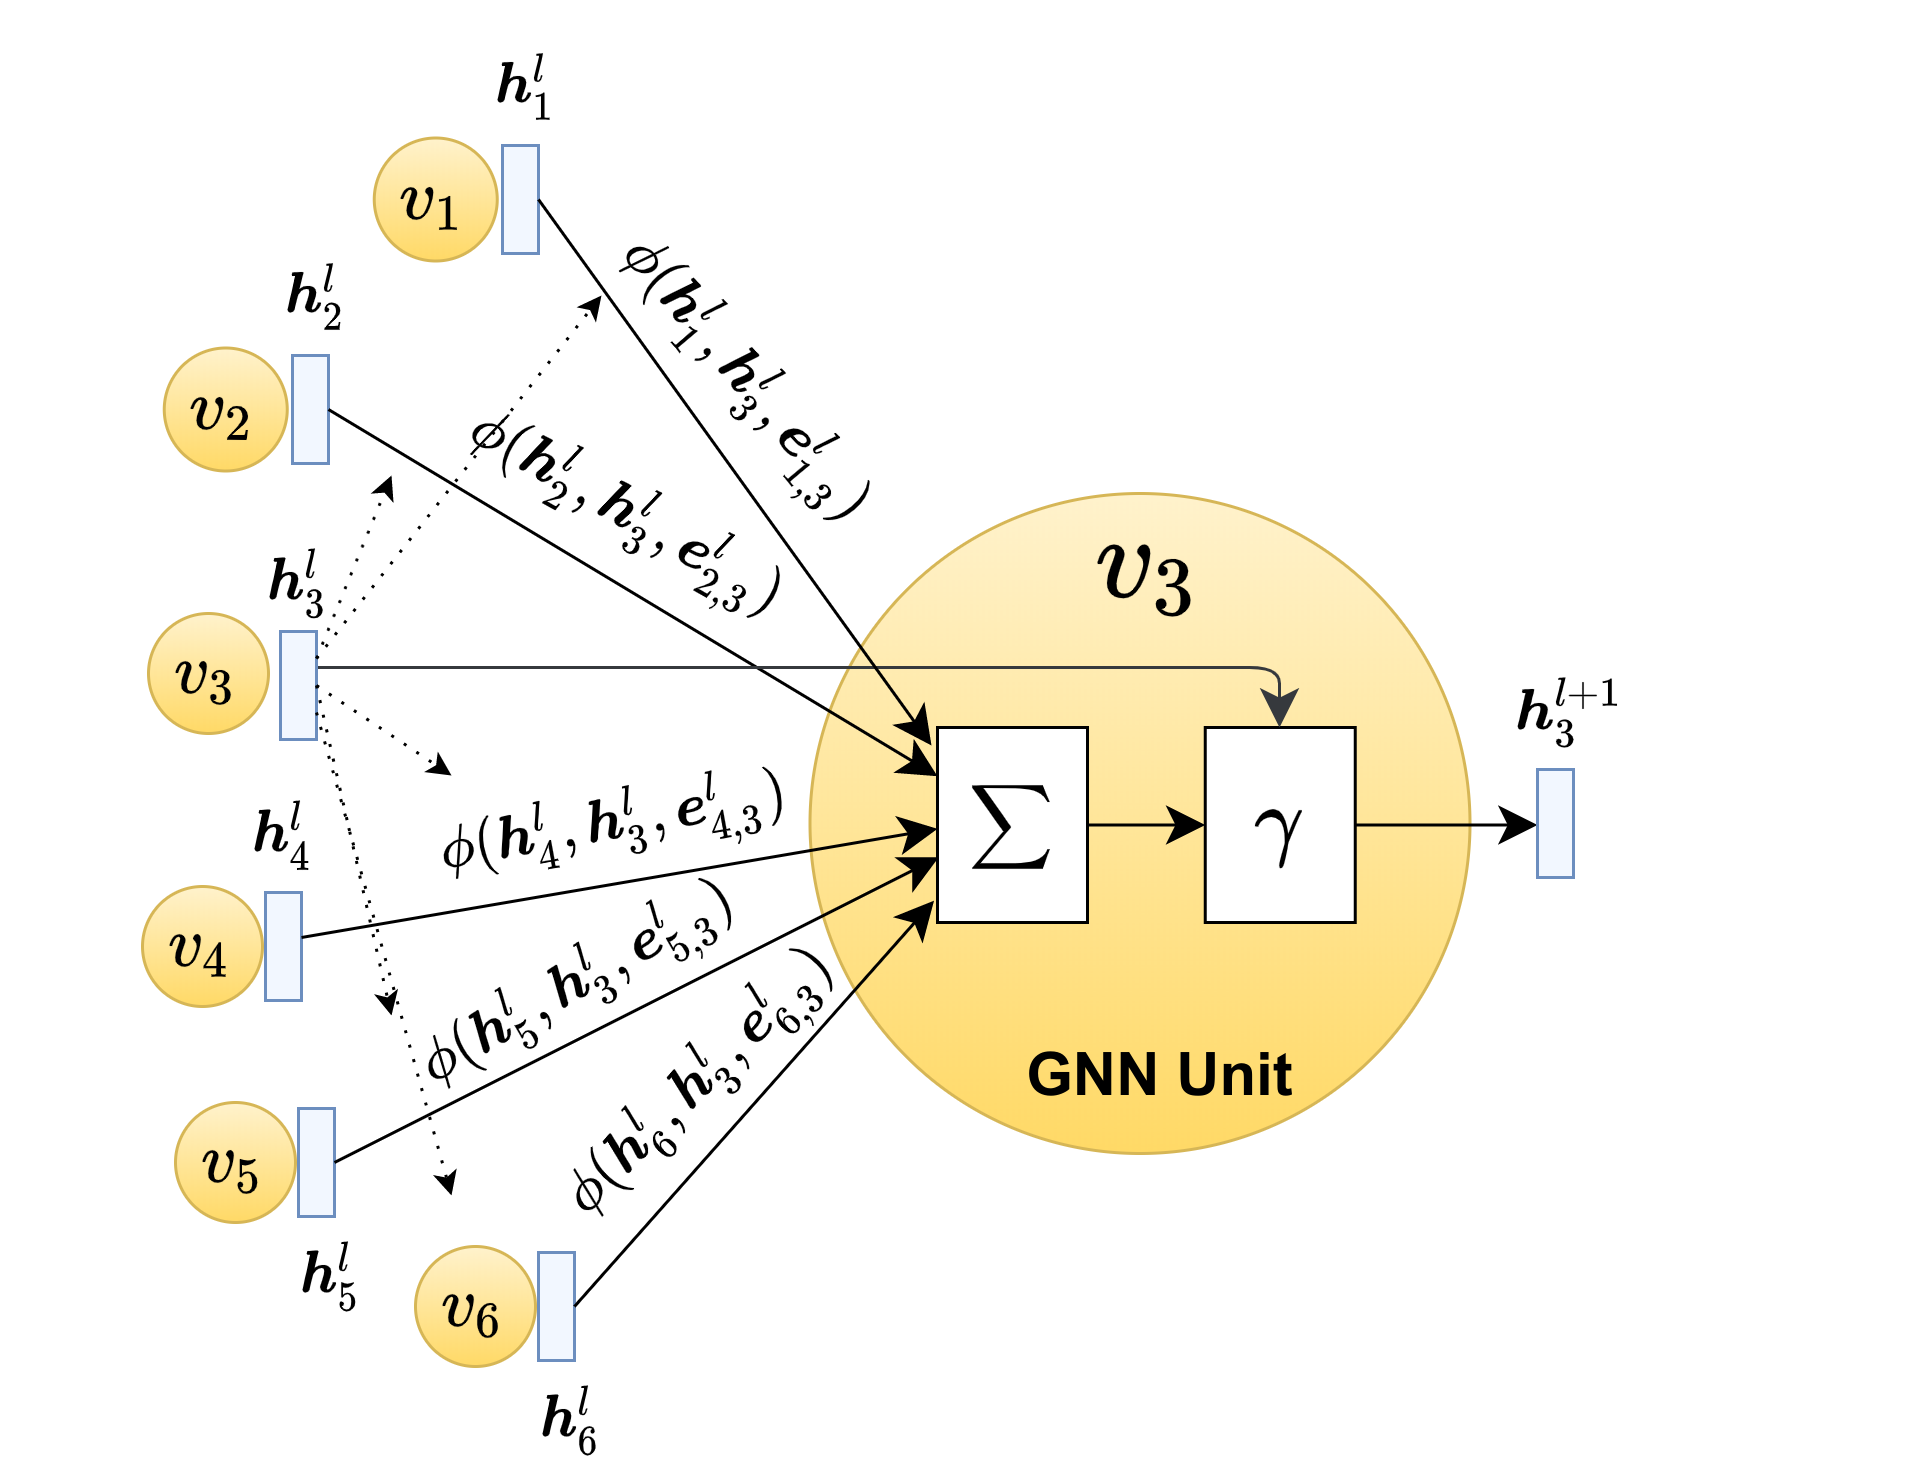
\includegraphics[width=0.6\columnwidth]{figs/illustration/GNN_Unit.png}
	\caption{Graph neuron of $v_3$ at the GNN layer $l$ with the graph $\mathcal{G}$ in \figurename~\ref{fig:general_structure_of_gnn}(b). $\phi$/$\Sigma$/$\gamma$ are the message/aggregation/vertex update functions in the message-passing model, respecitvely.}
	\label{fig:graph_neuron_structure}
\end{figure}

We follow the message-passing model \cite{gilmer_messgae_passing} to formally define a graph neuron.
The message-passing model is widely used in the cutting-edge GNN training systems like PyTorch Geometric (PyG) \cite{PyG} and Deep Graph Library (DGL) \cite{DGL}.
\figurename~\ref{fig:graph_neuron_structure} shows the structure of a graph neuron in the message-passing model.
Graph neurons at layer $l$ are made of three \emph{differentiable} functions: $\phi^l$, $\Sigma^l$ and $\gamma^l$.
The graph neuron calculates the output hidden vector $\boldsymbol{h}^{l+1}_i$ by
$$
\boldsymbol{h}^{l+1}_i = \gamma^l(\boldsymbol{h}^l_i, \mathlarger{\Sigma}^l_{v_j \in \mathcal{N}(v_i)}{\phi^l(\boldsymbol{h}^l_i, \boldsymbol{h}^l_j,	\boldsymbol{e}_{j,i})}).
$$

$\phi^l$ is the \emph{message} function.
For every incident edge $(v_j, v_i)$ of $v_i$, $\phi$ receives the output hidden feature vectors $\boldsymbol{h}^l_i$ and $\boldsymbol{h}^l_j$ of the previous GNN layer and the edge feature vector $\boldsymbol{e}_{j,i}$ as the input.
$\phi^l$ outputs a message vector $\boldsymbol{m}^l_{j,i}$ for every edge $(v_j, v_i)$ at layer $l$, i.e., $\boldsymbol{m}^l_{j,i}=\phi^l(\boldsymbol{h}^l_i, \boldsymbol{h}^l_j, \boldsymbol{e}_{j,i})$.
For $v_i$, the message vectors $\boldsymbol{m}^l_{x,j}$ with $v_x \in \mathcal{N}(v_i)$ are aggregated by the \emph{aggregation} function $\Sigma^l$ to produce an aggregated vector $\boldsymbol{s}^l_i$, i.e., $\boldsymbol{s}^l_i=\mathlarger{\Sigma}^l_{v_j \in \mathcal{N}(v_i)}\boldsymbol{m}^l_{j,i}$.
$v_i$'s aggregated vector $\boldsymbol{s}^l_i$ and its hidden vector $\boldsymbol{h}^l_i$ from the previous GNN layer are fed into the \emph{vertex update} function $\gamma^l$ to calculate the output hidden vector $\boldsymbol{h}^{l+1}_i$ of the current layer $l$, i.e., $\boldsymbol{h}^{l+1}_i = \gamma^l(\boldsymbol{h}^l_i, \boldsymbol{s}^l_i)$
The end-to-end training requires $\phi^l$ and $\gamma^l$ (like multi layer perceptrons and GRU) and $\Sigma_l$ (like mean, sum, element-wise min/max) are \emph{differentiable} to make the whole GNN differentialble.

Different GNNs adopt different kinds of graph neurons and have different definitions of the three functions.
$\phi$ and $\Sigma$ are the \emph{edge computation} functions.
They are conducted over every edge in $\mathcal{G}$.
$\gamma$ is the \emph{vertex computation} function.
It is conducted over every vertex in $\mathcal{G}$.
\tablename~\ref{tab:gnn_overview_edge} and \tablename~\ref{tab:gnn_overview_vertex} list the edge functions and the vertex functions of typical GNNs, respectively.
For ChebNet, we report its GNN layer in the tables \footnote{A layer of ChebNet consists of $K$ GNN sub-layers and a summation layer, i.e., $\boldsymbol{H}^{l+1} = \sum_{k=1}^K{\boldsymbol{Z}^{(k)} \textcolor{blue}{\boldsymbol{W}^{(k)}}}$ with GNN layers $\boldsymbol{Z}^{(1)}=\boldsymbol{H}$, $\boldsymbol{Z}^{(2)}=\hat{\boldsymbol{L}}\boldsymbol{H}$, and $\boldsymbol{Z}^{(k)}=2\hat{\boldsymbol{L}}\boldsymbol{Z}^{(k-1)} - \boldsymbol{Z}^{(k-2)}$. $\boldsymbol{H}^l$ is the matrix of output hidden feature vectors of the layer $l-1$. In the table, we report the GNN sub-layer of ChebNet that calculates $\boldsymbol{Z}^{(k)}$}.

\begin{table}
	\hspace{-10em}
    \begin{footnotesize}
        \begin{tabular}{ccp{8em}p{22em}r}
		\toprule
		GNN &
		Type &
		$\Sigma$ &
		$\phi$ &
		Complexity \\ \midrule
		ChebNet \cite{defferrad2016_chebnet} &
		Spectral &
		sum &
		$\boldsymbol{m}_{j, i}^{(k)} = e_{j, i}\boldsymbol{z}_j^{(k-1)}$ &
		$O(d_{in})$ \\
		\textbf{GCN} \cite{kipf2017_gcn} &
		Spectral &
		sum &
		$\boldsymbol{m}_{j, i}^l = e_{j, i} \boldsymbol{h}_j^l$ &
		$O(d_{in})$ \\
		AGCN &
		Spectral &
		sum &
		$\boldsymbol{m}_{j, i}^l = \tilde{e}_{j, i}^l \boldsymbol{h}_j^l$ &
		$O(d_{in})$ \\
		GraphSAGE &
		Non-spectral &
		mean/LSTM &
		$\boldsymbol{m}_{j, i}^l =  \boldsymbol{h}_j^l$ &
		$O(1)$ \\
		GraphSAGE-pool &
		Non-spectral &
		max &
		$\boldsymbol{m}_{j, i}^l =  \delta(\textcolor{blue}{\boldsymbol{W}^l_{pool}} \boldsymbol{h}_j^l + \textcolor{blue}{b}^l)$  &
		$O(d_{in} * d_{out})$ \\
		Neural FPs &
		Non-spectral &
		sum &
		$\boldsymbol{m}_{j, i}^l = \boldsymbol{h}_j^l$ &
		$O(1)$ \\
		SSE &
		Recurrent &
		sum &
		$\boldsymbol{m}_{j, i}^l = [\boldsymbol{h}_i^{l} \parallel \boldsymbol{h}_j^l]$ &
		$O(d_{in})$ \\
		\textbf{GGNN} &
		Gated &
		sum &
		$\boldsymbol{m}_{j, i} = \textcolor{blue}{\boldsymbol{W}^l} \boldsymbol{h}_j^l$ &
		$O(d_{in} * d_{out})$ \\
		\textbf{GAT}&
		Attention &
		sum  &
		\begin{scriptsize}
			$\begin{aligned}[t]
			& \alpha_{j, i}^k = \frac {\exp(LeakyReLU(\textcolor{blue}{\boldsymbol{a}^T} [ \textcolor{blue}{\boldsymbol{W}^{l,k}}  \boldsymbol{h}_j^l \parallel \textcolor{blue}{\boldsymbol{W}^{l,k}}  \boldsymbol{h}_j^l] ))} {\sum_{k \in \mathcal{N}(i)}\exp(LeakyReLU(\textcolor{blue}{\boldsymbol{a}^T} [ \textcolor{blue}{\boldsymbol{W}^{l,k}}  \boldsymbol{h}_j^l \parallel \textcolor{blue}{\boldsymbol{W}^{l,k}}  \boldsymbol{h}_k^l] ))} \\
			& Multi-head\ concatenation: \boldsymbol{m}_{j, i}^l = \parallel_{k=1}^K \delta(\alpha_{j, i}^k \textcolor{blue}{\boldsymbol{W}^{l,k}} \boldsymbol{h}_j^{l}) \\
			& Multi-head\ average: \boldsymbol{m}_{j, i}^l = \frac{1}{K} \sum_{k=1}^K \delta(\alpha_{j, i}^k \textcolor{blue}{\boldsymbol{W}^{l,k}} \boldsymbol{h}_j^{l})
			\end{aligned}$
		\end{scriptsize} &
		$O(K * d_{in} * d_{out})$ \\
		\textbf{GaAN} &
		Attention &
		sum,max,mean &
		\begin{scriptsize}
			$\begin{aligned}[t]
			&\alpha_{j, i}^k = \frac {\exp(\textcolor{blue}{\boldsymbol{a}^T} [ \textcolor{blue}{\boldsymbol{W}^{l, k}_{xa}} \boldsymbol{h}_j^l \parallel \textcolor{blue}{\boldsymbol{W}^{l,k}_{ya}} \boldsymbol{h}_i^l] )} {\sum_{k \in \mathcal{N}(j)}\exp(\textcolor{blue}{\boldsymbol{a}^T} [ \textcolor{blue}{\boldsymbol{W}^{l,k}_{xa}} \boldsymbol{h}_j^l \parallel \textcolor{blue}{\boldsymbol{W}^{l,k}_{ya}}  \boldsymbol{h}_k^l] )} \\
			&\boldsymbol{m}_{j, i, 1}^l = \parallel_{k=1}^K \delta(\alpha_{j, i}^k \textcolor{blue}{\boldsymbol{W}^{l,k}_v} \boldsymbol{h}_j^{l}) \\
			&\boldsymbol{m}_{j, i, 2}^l = \textcolor{blue}{\boldsymbol{W}^l_m} \boldsymbol{h}_j^{l} \\
			&\boldsymbol{m}_{j, i, 3}^l = \boldsymbol{h}_j^l
			\end{aligned}$
		\end{scriptsize} &
		$O(max(d_a, d_m, d_v) * K * d_{in})$ \\
		\bottomrule
	\end{tabular}
\end{footnotesize}
	\caption{Typical graph neural networks and their edge computation functions.$d_{in}$ and $d_{out}$ are dimensions of the input and output hidden feature vectors, respectively.
		Blue variables are model parameters to learn. For ChebNet, we report its GNN sub-layer. Because two sum operator are interchangeable and sum operator and concatenation operator are interchangeable, we do it for GAT to explain more clearly in edge computations functions.}
	\label{tab:gnn_overview_edge}
\end{table}

\begin{table}
	\hspace{-3em}
    \begin{footnotesize}
        \begin{tabular}{cp{20em}r}
		\toprule
		GNN &
		$\gamma$ &
		Complexity \\ \midrule
		ChebNet \cite{defferrad2016_chebnet} &
		$\boldsymbol{z}_i^{(k)} = 2\boldsymbol{s}^{(k)}_{i} - \boldsymbol{z}_i^{(k-2)}$&
		$O(d_{in})$ \\
		\textbf{GCN} \cite{kipf2017_gcn} &
		$\boldsymbol{h}_i^{l+1} = \textcolor{blue}{\boldsymbol{W}}^l  \boldsymbol{s}_i^{l}$ &
		$O(d_{in} * d_{out})$ \\
		AGCN &
		$\boldsymbol{h}_i^{l+1} = \textcolor{blue}{\boldsymbol{W}}^l  \boldsymbol{s}_i^{l}$ &
		$O(d_{in} * d_{out})$ \\
		GraphSAGE &	
		$\boldsymbol{h}_i^{l+1} =   \delta(\textcolor{blue}{\boldsymbol{W}}^l  [\boldsymbol{s}_i^{l} \parallel \boldsymbol{h}_i^l])$ &
		$O(d_{in} * d_{out})$ \\
		GraphSAGE-pool &	
		$\boldsymbol{h}_i^{l+1} = \boldsymbol{s}_i^l$ &
		$O(1)$ \\
		Neural FPs &
		$\boldsymbol{h}_i^{l+1} = \delta(\boldsymbol{h}_i^l + \textcolor{blue}{\boldsymbol{W}}^{l, |\mathcal{N}(i)|}  \boldsymbol{s}_i^{l})$ &
		$O(d_{in} * d_{out})$ \\
		SSE &
		$\boldsymbol{h}_i^{l+1} = (1 - \alpha)  \boldsymbol{h}_i^l +\alpha    \delta(\textcolor{blue}{\boldsymbol{W}}^l_1 \delta(\textcolor{blue}{\boldsymbol{W}}^l_2 \boldsymbol{s}_i^l))$ &
		$O(d_{in} * d_{out})$ \\
		\textbf{GGNN} &
		\begin{scriptsize}
		$\begin{aligned}[t]
			& \textcolor{blue}{\boldsymbol{z}}_i^l = \delta ( \textcolor{blue}{\boldsymbol{W}}^z \boldsymbol{s}_i^l + \textcolor{blue}{\boldsymbol{b}}^{sz} + \textcolor{blue}{\boldsymbol{U}}^z \boldsymbol{h}_i^{l} + \textcolor{blue}{\boldsymbol{b}}^{hz}) \\ 
			&\boldsymbol{r}_i^l = \delta ( \textcolor{blue}{\boldsymbol{W}}^r \boldsymbol{s}_i^l+ \textcolor{blue}{\boldsymbol{b}}^{sr} +\textcolor{blue}{\boldsymbol{U}}^r \boldsymbol{h}_i^{l} + \textcolor{blue}{\boldsymbol{b}}^{hr}) \\ 
			&\boldsymbol{h}_i^{l+1} = tanh ( \textcolor{blue}{\boldsymbol{W}} \boldsymbol{s}_i^l + \textcolor{blue}{\boldsymbol{b}}^s + \textcolor{blue}{\boldsymbol{U}} ( \boldsymbol{r}_i^l \odot \boldsymbol{h}_i^{l} + \textcolor{blue}{\boldsymbol{b}}^h))) \\ 
			&\boldsymbol{h}_i^{l+1} = (1 - \textcolor{blue}{\boldsymbol{z}}_i^l) \odot \boldsymbol{h}_i^l +  \textcolor{blue}{\boldsymbol{z}}_i^l \odot \boldsymbol{h}_i^{l+1}
		\end{aligned}$
		\end{scriptsize}
		&
		$O(max(d_{in}, d_{out}) * d_{out})$ \\
		\textbf{GAT}&
		$\boldsymbol{h}_i^{l+1} = \boldsymbol{s}_i^l$ &
		$O(1)$ \\
		\textbf{GaAN} &
		\begin{scriptsize}
			$\begin{aligned}[t]
			&\boldsymbol{g}_i = \textcolor{blue}{\boldsymbol{W}}^l_g  [\boldsymbol{h}_i^{l} \parallel \boldsymbol{s}_{i, 2}^l \parallel \boldsymbol{s}_{i, 3}^l]  \\
			&\boldsymbol{h}_i^{l+1} = \textcolor{blue}{\boldsymbol{W}}^l_o [\boldsymbol{h}_i^l \parallel (\boldsymbol{g}_{i} \odot \boldsymbol{s}_{i, 1}^l) ]
			\end{aligned}$ 
		\end{scriptsize}&
		$O(max(K * d_v + d_{in}, 2 * d_{in} + d_m) * d_{out})$ \\ \bottomrule
	\end{tabular}
\end{footnotesize}
	\caption{Typical graph neural networks and their vertex computation functions. $d_{in}$ and $d_{out}$ are dimensions of the input and output hidden feature vectors, respectively. Blue variables are model parameters to learn. For ChebNet, we report its GNN sub-layer.For Neural FPs, $\textcolor{blue}{\boldsymbol{W}}^{l, |\mathcal{N}(i)|}$ is the weight matrix for nodes with degree
	$|\mathcal{N}(i)|$ at layer $l$.}
	\label{tab:gnn_overview_vertex}
\end{table}

\subsection{Classification of GNNs}

Since we focus on analyzing the performance bottleneck in training GNNs, we classify the typical GNNs from the view of computational complexity.
The computational complexity of a GNN layer is related to the complexity of its vertex and edge functions, i.e. $O(m * (O_\phi + O_\Sigma) + n * O_\gamma)$, where $O_\phi$/$O_\Sigma$/$O_\gamma$ are the computational complexity of the three functions.

The complexity can be decomposed into two parts: the edge computation complexity $O_\phi$ + $O_\Sigma$ and the vertex computation complexity $O_\gamma$.
In \tablename~\ref{tab:gnn_overview_edge} and \tablename~\ref{tab:gnn_overview_vertex}, we list the edge and vertex computation complexity, respectively.
The edge/vertex complexity of a graph neuron are affected by the dimensions of the input/output hidden vectors $d_{in}$ and $d_{out}$ and the dimensions of the model parameters (like the number of heads $K$ in GAT and the dimensions of the view vectors $d_a$/$d_v$ in GaAN).

We classify the typical GNNs into four quadrants based on their edge/vertex complexity as shown in \figurename~\ref{fig:gnn_complexity_quadrant}. We pick GCN, GGNN, GAT and GaAN as the representative GNNs of the four quadrants.

\begin{figure}
	\centering
	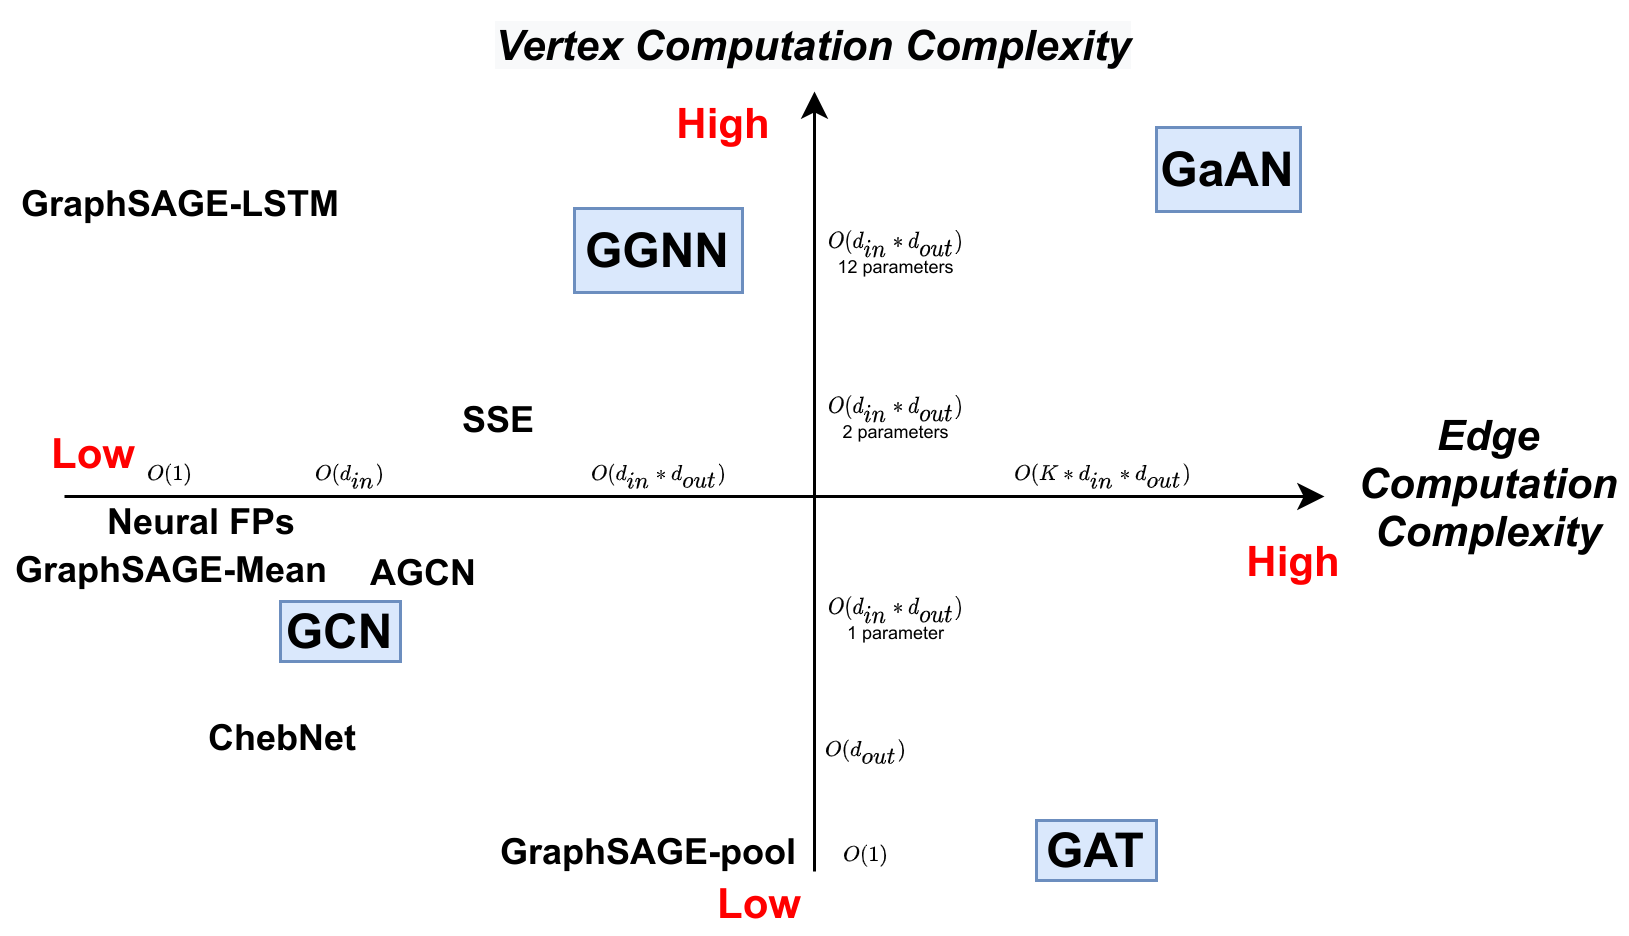
\includegraphics[width=0.7\columnwidth]{figs/illustration/GNN_complexity_quadrant.png}
	\caption{Complexity quadrants of typical GNNs. If two GNNs have the same complexity under the Big-O notation, we further compare their complexity according to how many parameters they need to train.}
	\label{fig:gnn_complexity_quadrant}
\end{figure}

\textbf{GCN} \cite{kipf2017_gcn} (low vertex \& edge computational complexity): Graph convolution network (GCN) is the first-order approximation of the spectral-based graph convolutions.
%By combining the advantages of both the spectral-based and the spatial-based convolution, it can learn the representation of the local topological structure and vertex features efficiently.
It has only one parameter to learn at each layer, i.e. the weight matrix $\boldsymbol{W}^l$ in $\gamma$.
A GCN graph neuron can be expressed as $\boldsymbol{h}^{l+1}_i = \boldsymbol{W}^l\sum_{v_j \in \mathcal{N}(v_i)}{e_{j,i}\boldsymbol{h}^l_j}$, where $e_{j,i}$ is the normalized weight of the edge $(v_j, v_i)$.
%In the matrix view, $\boldsymbol{H}^{l+1} = (\boldsymbol{A}\boldsymbol{H}^l)\boldsymbol{W}^l$.
According to the associative law of the matrix multiplication, $\boldsymbol{h}^{l+1}_i = \sum_{v_j \in \mathcal{N}(v_i)}{e_{j,i}\boldsymbol{W}^l\boldsymbol{h}^l_j}$.
Since the dimension of $\boldsymbol{h}^{l+1}_i$ is usually smaller than $\boldsymbol{h}^l_i$ in practical GCNs, the implementation of GCN \footnote{The implementation of GCN in PyTorch Geometric: \url{ https://github.com/rusty1s/pytorch_geometric/blob/1.5.0/torch_geometric/nn/conv/gcn_conv.py}} chooses to first conduct the vertex computation $\hat{\boldsymbol{h}}^l_j = \boldsymbol{W}^l\boldsymbol{h}^l_j$ for each vertex $v_j$ and then conduct the edge computation $\boldsymbol{h}^{l+1}_i=\sum_{v_j\in\mathcal{N}(v_i)}{\hat{\boldsymbol{h}}^l_j}$.
As $\hat{\boldsymbol{h}}^l_j$ has the same dimension as $\boldsymbol{h}^{l+1}_i$, the implementation significantly reduces the  computation cost of the edge computation.